\documentclass[11pt]{article}

\usepackage[letterpaper,margin=1in]{geometry}
\usepackage[T1]{fontenc}
\usepackage{lmodern}
\usepackage{microtype}
\usepackage{graphicx}
\usepackage{booktabs}
\usepackage{tabularx}
\usepackage{enumitem}
\usepackage{xurl}
\usepackage{hyperref}

\hypersetup{hidelinks}
\setlist{itemsep=2pt,parsep=0pt,topsep=6pt,partopsep=0pt}
\graphicspath{{uml/rendered/}}
\setlength{\parskip}{6pt plus 1pt minus 1pt}
\setlength{\parindent}{0pt}
\setlength{\emergencystretch}{5em}
\pagestyle{plain}
\urlstyle{same}

\title{Market Intelligence Agent}
\author{}
\date{}

\begin{document}

\begin{titlepage}
\centering
\vspace*{0.75in}
{\Large York University\\[0.15em]}
{\large Lassonde School of Engineering\\[2.4em]}
{\Large EECS3311 -- Software Design\\[2.6em]}
{\Huge\bfseries Market Intelligence Agent\\[0.55em]}
{\Large Stage 2 -- Implementation\\[2.15in]}
\begin{tabular}{rl}
\textbf{Student:} & [Erdem Calikoglu] \\
\textbf{Student Number:} & [218188771] \\
\textbf{Instructor:} & [Song Wang] \\
\textbf{Date:} & [November 5, 2026] \\
\end{tabular}
\vfill
\end{titlepage}

\tableofcontents
\newpage

\section{Project Description and Scope}

\subsection{Project Title}
Market Intelligence Agent

\subsection{Project Description}
The Market Intelligence Agent is a Java 21 research desk for a signed-in user. The same services answer the Swing window and the terminal. Accounts, portfolios, watchlists, and conversation turns are stored in one SQLite database, \texttt{data/market-intelligence.db}. The desk retrieves quotes, company profiles, ETF exposure, news, statements, price history, and a sentiment score, and it can write a short note about a price move. It does not give investment advice. A movement note and a follow-up reply say so.

Stage~1 described this system as a design. This report describes the application that is in the repository. A feature listed here has a class and a command. A limit is stated as the behavior of the running desk, not as a plan for a later change.

Market data comes from free provider plans. \texttt{ProviderRouter} selects the first adapter registered for a capability. A later adapter is used only when an earlier one was not registered. A failed call does not try the next adapter. Keys are environment variables. The process does not read a \texttt{.env} file. \texttt{.env.example} contains placeholders only.

Gemini participates in two places. \texttt{MarketExplanationService} writes a short note from a quote and up to three headlines. \texttt{RequestPlanner} may ask Gemini to name one allowlisted action for a sentence, and \texttt{AgentController} may ask it for a short reply from the tool result. A direct command such as \texttt{QUOTE NVDA} does not call the model. Portfolio weights are calculated in Java and are not sent to Gemini. If the model returns bad JSON, a disallowed action, or a word that is not a ticker, the keyword plan is used.

The default model is \texttt{gemini-3.5-flash-lite}. \texttt{GEMINI\_MODEL} overrides it. \texttt{gemini-3.8-flash} thought too long for a short note. \texttt{gemini-2.5-flash} returned HTTP 404 for a new key. Those names stay unset.

The project is not a brokerage and it does not place orders. Its scope is financial-information retrieval, ETF and portfolio analysis, news retrieval, and an explanation grounded in the quote and the headlines that were retrieved.

\section{Implementation Status}

The following behavior is in the repository on 5~November 2026.

\begin{itemize}
\item Register, sign in, and sign out, on separate GUI screens and in the terminal.
\item Quotes, company overviews, security comparison, news, ETF sector weights, ETF overlap, portfolio view, portfolio edits, and watchlists.
\item Country exposure: the published Finnhub report when the plan allows it, otherwise the headquarters country of at most 25 holdings.
\item Portfolio exposure as price times quantity, with currencies kept apart.
\item A movement explanation from the quote and the news, with a Gemini note when the key is set.
\item Follow-up questions that remember the last symbol for that user only.
\item Annual statements, daily bars with a 14-day RSI, and one sentiment score, when those keys are set.
\item A home screen with portfolio value, day move, position chips, and a quote and news tape.
\end{itemize}

The following limits are part of the implementation.

\begin{itemize}
\item Period~1 (20--26 October 2026) has no commits in this repository. That week cannot be repaired by later commits, and those commits were not backdated.
\item Period~3 (3--9 November 2026) has six non-merge commits. Five of them change the desk and meet the minimum of five meaningful code commits. They are listed under Weekly Commits.
\item Demonstration videos do not yet have public links. Section~\ref{sec:demos} is the index. Recordings of the flows that do not call a vendor were captured with this report. Live provider clips still need the student's keys and a public link.
\item Country weights on the free plan are headquarters of reported holdings. They are not the fund's published country report and they are not revenue exposure. Unknown and unassigned weight is named. It is not filled in.
\item Finnhub's free plan prices US listings. A symbol such as \texttt{XEQT.TO} stays unpriced and is named.
\item Alpha Vantage company overview is a premium endpoint. This desk uses Alpha Vantage for ETF profile and holdings.
\item The router does not fail over when a live call fails.
\item The model cannot add or remove a position. Those commands stay on \texttt{SessionWorkspace}.
\item A sentence that tries to override the instructions is rejected and does not run a tool.
\end{itemize}

\section{Major Features}

\subsection{User Authentication}
The desk supports account registration, login, and logout. Passwords are not stored directly. \texttt{BCryptPasswordHasher} stores a hash. A username is 3 to 30 characters. A password is at least 8 characters. Registration returns to the sign-on screen. The user still has to log in. A failed login does not say whether the username or the password was wrong.

\subsection{Persistent User Profiles}
Each user has a portfolio and a watchlist in SQLite. Conversation turns are stored for that user id. Logging out clears the in-memory session. The rows remain under the previous user. The next person must sign in.

\subsection{Natural-Language Follow-Up}
A sentence that is not a slash command is a follow-up. \texttt{RequestPlanner} maps it to one allowlisted action. Pronouns use the last symbol stored for this user. \texttt{why did microsoft fall} stays a sentence: Microsoft maps to \texttt{MSFT}, and the word ``did'' is a stop word, so it cannot become the ticker. Compare and overlap still require two symbols. Portfolio edits are not on the allowlist.

\subsection{Terminal and Window Commands}
The terminal accepts slash commands. The window accepts the same verbs, with or without a leading slash, and the research buttons. Both call \texttt{ResearchGateway}. A successful lookup stores the symbol for a later follow-up.

\subsection{Market Data}
Quotes and company profiles come from Finnhub when \texttt{FINNHUB\_API\_KEY} is set. Twelve Data is the quote fallback and the source of daily bars and RSI. Alpha Vantage is the last quote fallback and the source of ETF holdings. A quote shows last price, previous close, and percent change. A direct quote does not call Gemini.

\subsection{ETF Exposure and Overlap}
Sector weights come from the ETF profile. Country exposure tries Finnhub's published report. On HTTP 403 the desk reads holdings and the headquarters country of at most 25 names. Overlap is the shared holdings of two ETFs. The calculations are in Java.

\subsection{News, Movement, Statements, History, and Sentiment}
News prefers Marketaux when its token is set, and otherwise uses Finnhub company news. A movement explanation needs a quote and news. Gemini writes the note from that evidence. Statements come from Financial Modeling Prep. History and RSI come from Twelve Data. The sentiment score comes from SentiSense. The display band is this desk's label for the score.

\subsection{Portfolio, Watchlist, and Home Desk}
A position stores a symbol, a quantity, and a type of \texttt{STOCK}, \texttt{ETF}, or \texttt{OTHER}. Exposure values each position as price times quantity. Currencies stay in separate books. The home screen shows that value, the day move, one chip per position, and a tape. The terminal lists the same positions with \texttt{/portfolio} and does not show a sliding tape.

\section{Major User Interactions}
The implementation supports twenty user-facing interactions. Login, logout, and registration are included because Stage~1 specified them. They are not counted toward the ten meaningful features. The meaningful features are UC-04 through UC-20.

\begin{enumerate}
\item UC-01 -- Register Account
\item UC-02 -- Log In
\item UC-03 -- Log Out
\item UC-04 -- Get Market Quote
\item UC-05 -- Get Security Overview
\item UC-06 -- Analyze ETF Exposure
\item UC-07 -- Compare Securities
\item UC-08 -- Analyze ETF Holding Overlap
\item UC-09 -- Retrieve Financial News
\item UC-10 -- Explain Recent Market Movement
\item UC-11 -- Add Portfolio Position
\item UC-12 -- Remove Portfolio Position
\item UC-13 -- View Portfolio
\item UC-14 -- Manage Watchlist
\item UC-15 -- Analyze Portfolio Exposure
\item UC-16 -- Ask a Contextual Follow-Up Question
\item UC-17 -- Read Financial Statements
\item UC-18 -- Read Price History
\item UC-19 -- Read Sentiment
\item UC-20 -- View Home Desk
\end{enumerate}

\section{Use Cases}

\subsection{UC-01 -- Register Account}
\textbf{Primary Actor:} User.

\textbf{Goal:} Create a new user account.

\textbf{Preconditions:} The application is running and SQLite is available.

\textbf{Trigger:} The user opens the create-account screen, or chooses register in the terminal.

\textbf{Main Success Scenario:}
\begin{enumerate}
\item The user enters a username and a password. The window also asks for a confirmation.
\item \texttt{AuthService.register} validates the lengths and the username characters.
\item The service checks that the username is not already stored.
\item \texttt{BCryptPasswordHasher} hashes the password.
\item \texttt{SQLiteUserRepository.save} stores the user. The password is not copied into the status line.
\item The window returns to the sign-on screen. The user is not signed in yet.
\end{enumerate}
\textbf{Alternative/Exception Flows:}
\begin{itemize}
\item A taken username, a short password, or a confirmation that does not match is rejected.
\item A persistence failure does not create the account.
\end{itemize}
\textbf{Postconditions:} A new user row exists. No session is active.

\textbf{Classes and patterns:} \texttt{AuthenticationPanel}, \texttt{TerminalUI}, \texttt{SessionWorkspace}, \texttt{AuthService}, \texttt{PasswordHasher}. Strategy, Repository, and Factory (\texttt{ApplicationContext} wires them). Deterministic.

\subsection{UC-02 -- Log In}
\textbf{Primary Actor:} User.

\textbf{Goal:} Start a session for an existing account.

\textbf{Preconditions:} The user has registered.

\textbf{Trigger:} The user submits a username and password on the sign-on screen. That screen has no confirmation field.

\textbf{Main Success Scenario:}
\begin{enumerate}
\item \texttt{AuthService.authenticate} loads the user by username.
\item The hasher checks the password against the stored hash.
\item \texttt{SessionManager} starts a session for that user id.
\item The window opens the desk. The terminal opens the authenticated prompt.
\end{enumerate}
\textbf{Alternative/Exception Flows:} A mismatch stays on the sign-on screen and does not say which field failed.

\textbf{Postconditions:} An authenticated session exists for that user id.

\textbf{Classes and patterns:} \texttt{AuthenticationPanel} or \texttt{TerminalUI}, \texttt{AuthService}, \texttt{SessionManager}. Strategy and Repository. Deterministic.

\subsection{UC-03 -- Log Out}
\textbf{Primary Actor:} Authenticated user.

\textbf{Goal:} End the active session.

\textbf{Preconditions:} A user is signed in.

\textbf{Trigger:} The user chooses logout.

\textbf{Main Success Scenario:}
\begin{enumerate}
\item \texttt{SessionWorkspace.logout} calls \texttt{SessionManager.endSession}.
\item In-memory session state is cleared.
\item The next command requires sign-on.
\end{enumerate}
\textbf{Postconditions:} No authenticated session remains. Conversation rows stay in SQLite under the previous user id.

\textbf{Classes and patterns:} \texttt{SessionWorkspace}, \texttt{SessionManager}. Facade. Deterministic.

\subsection{UC-04 -- Get Market Quote}
\textbf{Primary Actor:} Authenticated user.

\textbf{Goal:} Show the latest price, previous close, and percent change.

\textbf{Preconditions:} A quote adapter is registered. The order is Finnhub, then Twelve Data, then Alpha Vantage.

\textbf{Trigger:} \texttt{QUOTE NVDA} or \texttt{/quote NVDA}.

\textbf{Main Success Scenario:}
\begin{enumerate}
\item \texttt{ResearchGateway} checks that the signed-in user still matches the request.
\item \texttt{MarketDataTool} validates the symbol and calls \texttt{ProviderRouter.getQuote}.
\item The first registered quote adapter returns a \texttt{MarketQuote}.
\item The window or the terminal shows the price, the previous close, and the percent change.
\item The symbol is stored as the last lookup for this user.
\end{enumerate}
\textbf{Alternative/Exception Flows:} A blank or invalid symbol is rejected. A missing key says which variable to set. Gemini is not called. Stage~1 sent this use case through the model. That path was removed so a quote stays a lookup.

\textbf{Postconditions:} The user sees a retrieved quote or an explicit failure. The stored portfolio is unchanged.

\textbf{Classes and patterns:} \texttt{DeskCommand}, \texttt{CommandParser}, \texttt{MarketDataTool}, \texttt{FinnhubAdapter}. Command, Facade, Composite, Adapter. Deterministic.

\subsection{UC-05 -- Get Security Overview}
\textbf{Primary Actor:} Authenticated user.

\textbf{Goal:} Show the name, exchange, currency, and industry label.

\textbf{Preconditions:} Finnhub or Alpha Vantage is registered for overviews.

\textbf{Trigger:} \texttt{OVERVIEW NVDA}.

\textbf{Main Success Scenario:}
\begin{enumerate}
\item The same gateway and \texttt{MarketDataTool} call \texttt{getSecurityOverview}.
\item Finnhub's free profile supplies the name, exchange, currency, and a Finnhub industry label.
\item The screen says that the profile has no company description and no separate GICS sector.
\end{enumerate}
\textbf{Alternative/Exception Flows:} An ETF often has no company profile. Portfolio exposure then values it from the quote currency and names that fact. Alpha Vantage overview is a premium endpoint and returns that error when it is the only overview adapter.

\textbf{Postconditions:} The user receives an overview or an explicit failure.

\textbf{Classes and patterns:} Same quote path, with \texttt{ProviderRouter.getSecurityOverview}. Deterministic.

\subsection{UC-06 -- Analyze ETF Exposure}
\textbf{Primary Actor:} Authenticated user.

\textbf{Goal:} Show sector weights, or country weights, for one ETF.

\textbf{Preconditions:} Sector weights need \texttt{ALPHA\_VANTAGE\_API\_KEY}. Country weights need Finnhub, and the headquarters fallback also needs Alpha Vantage holdings.

\textbf{Trigger:} \texttt{SECTOR QQQ} or \texttt{GEO QQQ}.

\textbf{Main Success Scenario:}
\begin{enumerate}
\item \texttt{ETFExposureTool} loads the ETF profile and \texttt{ExposureCalculator} sums the provider's sector weights.
\item For country exposure, the tool requests Finnhub's published report.
\item On HTTP 403 it reads holdings and the headquarters country of at most 25 names through \texttt{HoldingCountryResolver}.
\item A holding with no profile is Unknown. Weight the provider left blank stays unassigned and is named.
\end{enumerate}
\textbf{Alternative/Exception Flows:} A stock such as \texttt{NVDA} has no holdings list, so it has no country breakdown. Provider errors pass through \texttt{ProviderText.redact}. Stage~1 had the model explain the exposure. The implementation shows the calculated weights instead.

\textbf{Postconditions:} A deterministic exposure result is shown, or the missing report is named.

\textbf{Classes and patterns:} \texttt{ETFExposureTool}, \texttt{AlphaVantageAdapter}, \texttt{FinnhubMarketDataClient}. Command, Adapter, Composite. Deterministic.

\subsection{UC-07 -- Compare Securities}
\textbf{Primary Actor:} Authenticated user.

\textbf{Goal:} Show the difference between two percent changes.

\textbf{Preconditions:} A quote adapter is registered. Two symbols are required.

\textbf{Trigger:} \texttt{COMPARE NVDA MSFT}.

\textbf{Main Success Scenario:}
\begin{enumerate}
\item \texttt{ComparisonTool} loads both quotes.
\item \texttt{SecurityComparisonCalculator} subtracts the second percent change from the first.
\item The screen shows both quotes and the difference.
\end{enumerate}
\textbf{Alternative/Exception Flows:} One symbol is rejected. A follow-up that names only one symbol asks for the second.

\textbf{Postconditions:} A structured comparison is displayed, or the failure is explicit.

\textbf{Classes and patterns:} \texttt{ComparisonTool}, \texttt{ProviderRouter}. Command, Composite, Adapter. Deterministic.

\subsection{UC-08 -- Analyze ETF Holding Overlap}
\textbf{Primary Actor:} Authenticated user.

\textbf{Goal:} List holdings that two ETFs share.

\textbf{Preconditions:} \texttt{ALPHA\_VANTAGE\_API\_KEY} is set. Two ETF symbols are required.

\textbf{Trigger:} \texttt{OVERLAP QQQ SPY}.

\textbf{Main Success Scenario:}
\begin{enumerate}
\item \texttt{ComparisonTool} loads both holding lists through the router.
\item \texttt{ExposureCalculator.calculateOverlap} reports the shared names.
\end{enumerate}
\textbf{Alternative/Exception Flows:} A missing key or a missing holdings list is reported. The overlap is not estimated.

\textbf{Postconditions:} The user receives the deterministic overlap, or an explicit failure.

\textbf{Classes and patterns:} \texttt{ComparisonTool}, \texttt{ExposureCalculator}, \texttt{AlphaVantageAdapter}. Command, Adapter. Deterministic.

\subsection{UC-09 -- Retrieve Financial News}
\textbf{Primary Actor:} Authenticated user.

\textbf{Goal:} Show recent articles associated with a symbol.

\textbf{Preconditions:} \texttt{MARKETAUX\_API\_TOKEN} or \texttt{FINNHUB\_API\_KEY} is set.

\textbf{Trigger:} \texttt{NEWS NVDA}.

\textbf{Main Success Scenario:}
\begin{enumerate}
\item \texttt{NewsTool} calls \texttt{ProviderRouter.getNews}.
\item Marketaux is used when its token is set. Otherwise Finnhub company news is used.
\item The screen shows headlines. A match means the ticker was associated with the article.
\end{enumerate}
\textbf{Alternative/Exception Flows:} Alpha Vantage news exists on \texttt{AlphaVantageAdapter} and is not registered, because that free plan is about 25 calls a day. Association is not evidence that the article caused a price move.

\textbf{Postconditions:} The user sees the retrieved articles or an explicit failure.

\textbf{Classes and patterns:} \texttt{NewsTool}, \texttt{MarketauxAdapter}, \texttt{FinnhubAdapter}. Command, Composite, Adapter. Deterministic.

\subsection{UC-10 -- Explain Recent Market Movement}
\textbf{Primary Actor:} Authenticated user.

\textbf{Goal:} Show the quote, the news, and a short note grounded in that evidence.

\textbf{Preconditions:} A quote provider and a news provider are registered.

\textbf{Trigger:} \texttt{WHY MSFT}, or a follow-up sentence that plans \texttt{MARKET\_MOVEMENT}.

\textbf{Main Success Scenario:}
\begin{enumerate}
\item \texttt{MarketMovementTool} gathers the quote and the news.
\item \texttt{NewsTiming} marks an article published after the last trade when the quote has a trade time.
\item \texttt{MarketExplanationService.explain} calls \texttt{GeminiLLMClient.generateBrief}.
\item The prompt contains the quote and short article text. It does not ask for a buy or sell decision.
\item The screen shows the evidence, the note, and the line that this is not investment advice.
\end{enumerate}
\textbf{Alternative/Exception Flows:} If Gemini is unset, times out, or returns an error, the quote and the news still appear with the failure note.

\textbf{Postconditions:} The user receives the evidence and either a note or an explicit explanation failure.

\textbf{Classes and patterns:} \texttt{MarketMovementTool}, \texttt{MarketExplanationService}, \texttt{ResponseComposer}. Command, Adapter, Strategy (\texttt{LLMProvider}). Hybrid.

\subsection{UC-11 -- Add Portfolio Position}
\textbf{Primary Actor:} Authenticated user.

\textbf{Goal:} Store a position for the signed-in user.

\textbf{Preconditions:} The user is signed in.

\textbf{Trigger:} \texttt{PORT ADD NVDA 10 STOCK}, or the Portfolio screen.

\textbf{Main Success Scenario:}
\begin{enumerate}
\item \texttt{SessionWorkspace.addPosition} checks the session.
\item \texttt{PortfolioService} validates the symbol, the quantity, and the asset type.
\item \texttt{SQLitePortfolioRepository} stores the position for this user id.
\end{enumerate}
\textbf{Alternative/Exception Flows:} An invalid quantity or type is rejected. A sentence cannot add a position. Stage~1 exposed this as a tool the planner could call. The implementation keeps it off the allowlist.

\textbf{Postconditions:} The position belongs to the authenticated user's stored portfolio.

\textbf{Classes and patterns:} \texttt{PortfolioPanel}, \texttt{DeskCommand}, \texttt{PortfolioService}. Command, Repository, Facade. Deterministic.

\subsection{UC-12 -- Remove Portfolio Position}
\textbf{Primary Actor:} Authenticated user.

\textbf{Goal:} Delete one symbol from the signed-in portfolio.

\textbf{Preconditions:} The user is signed in.

\textbf{Trigger:} \texttt{PORT REMOVE NVDA}.

\textbf{Main Success Scenario:}
\begin{enumerate}
\item \texttt{SessionWorkspace.removePosition} calls \texttt{PortfolioService.removePosition}.
\item The repository deletes that symbol for this user.
\item The screen reports whether the symbol was present.
\end{enumerate}
\textbf{Alternative/Exception Flows:} A missing symbol is reported and the other positions stay. The model cannot remove a position.

\textbf{Postconditions:} The requested position no longer exists when removal succeeds.

\textbf{Classes and patterns:} \texttt{PortfolioService}, \texttt{SQLitePortfolioRepository}. Command, Repository. Deterministic.

\subsection{UC-13 -- View Portfolio}
\textbf{Primary Actor:} Authenticated user.

\textbf{Goal:} List the stored positions.

\textbf{Preconditions:} The user is signed in.

\textbf{Trigger:} \texttt{/portfolio} or the Portfolio screen.

\textbf{Main Success Scenario:}
\begin{enumerate}
\item \texttt{PortfolioService.getPortfolio} loads the rows for this user.
\item The screen lists symbol, quantity, and asset type.
\end{enumerate}
\textbf{Alternative/Exception Flows:} An empty portfolio is shown as empty. Listing positions does not require a network call. Prices appear when another feature quotes them.

\textbf{Postconditions:} The stored portfolio is unchanged.

\textbf{Classes and patterns:} \texttt{PortfolioPanel}, \texttt{TerminalUI}, \texttt{SessionWorkspace}. Repository, Facade. Deterministic.

\subsection{UC-14 -- Manage Watchlist}
\textbf{Primary Actor:} Authenticated user.

\textbf{Goal:} Add or remove a symbol on the signed-in watchlist.

\textbf{Preconditions:} The user is signed in.

\textbf{Trigger:} \texttt{WATCH ADD NVDA} or \texttt{WATCH REMOVE NVDA}.

\textbf{Main Success Scenario:}
\begin{enumerate}
\item \texttt{WatchlistService} validates the symbol.
\item \texttt{SQLiteWatchlistRepository} stores or deletes it for this user.
\item The watchlist screen and \texttt{/watchlist} show the result.
\end{enumerate}
\textbf{Alternative/Exception Flows:} The watchlist has no quantity and is not a portfolio. Stage~1 had a \texttt{WatchlistTool} on the agent. The implementation uses the session workspace, as it does for portfolio edits.

\textbf{Postconditions:} The user's watchlist reflects the requested change.

\textbf{Classes and patterns:} \texttt{WatchlistPanel}, \texttt{WatchlistService}. Repository, Command. Deterministic.

\subsection{UC-15 -- Analyze Portfolio Exposure}
\textbf{Primary Actor:} Authenticated user.

\textbf{Goal:} Show sector weights by market value.

\textbf{Preconditions:} The user is signed in and a quote provider is registered.

\textbf{Trigger:} \texttt{EXPOSURE} or \texttt{/portfolio exposure}.

\textbf{Main Success Scenario:}
\begin{enumerate}
\item \texttt{PortfolioAnalysisTool} loads the signed-in positions.
\item Each position is quoted. Market value is price times quantity.
\item Day move is (price minus previous close) times quantity.
\item Currencies stay in separate books. A position with no price is excluded and named.
\item ETF sector weights are look-through when the holding list exists.
\end{enumerate}
\textbf{Alternative/Exception Flows:} \texttt{AgentController} does not ask Gemini to narrate this result, even when a sentence selects the action.

\textbf{Postconditions:} The user receives the calculated exposure. The stored quantities are unchanged.

\textbf{Classes and patterns:} \texttt{PortfolioAnalysisTool}, \texttt{PortfolioExposureCalculator}, \texttt{PortfolioBook}. Command, Composite, Adapter. Deterministic.

\subsection{UC-16 -- Ask a Contextual Follow-Up Question}
\textbf{Primary Actor:} Authenticated user.

\textbf{Goal:} Answer a sentence from the last stored symbol, or from a symbol named in the sentence.

\textbf{Preconditions:} The user is signed in. A pronoun requires an earlier lookup for this user.

\textbf{Trigger:} A sentence in the window follow-up field or at the terminal prompt, for example \texttt{what about its sector exposure}.

\textbf{Main Success Scenario:}
\begin{enumerate}
\item \texttt{ResearchGateway.ask} calls \texttt{AgentController.handle}.
\item \texttt{ConversationMemory.lastSymbol} reads recent turns for this user only.
\item \texttt{RequestPlanner.createPlan} builds a keyword plan. When Gemini is configured, it may replace that plan with one allowlisted JSON action.
\item \texttt{ToolManager} runs the action. \texttt{ResponseComposer} formats the tool result.
\item A second short model call may prepend a sentence. Both turns are stored.
\item The reply says that this is not investment advice.
\end{enumerate}
\textbf{Alternative/Exception Flows:}
\begin{itemize}
\item A sentence that tries to override the instructions does not run a tool.
\item Compare and overlap with one symbol ask for the second.
\item If Gemini is unset or returns a disallowed action, the keyword plan is used.
\item Portfolio exposure selected this way is not narrated by the model.
\end{itemize}
\textbf{Postconditions:} The conversation history for this user contains the question and the reply.

\textbf{Classes and patterns:} \texttt{AgentPanel}, \texttt{TerminalUI}, \texttt{RequestPlanner}, \texttt{PromptBuilder}, \texttt{ConversationMemory}. Command, Strategy, Facade, Repository. Hybrid when Gemini is set. Keyword-only when it is not.

\subsection{UC-17 -- Read Financial Statements}
\textbf{Primary Actor:} Authenticated user.

\textbf{Goal:} Show up to four annual periods of income, balance sheet, and cash flow.

\textbf{Preconditions:} \texttt{FMP\_API\_KEY} is set.

\textbf{Trigger:} \texttt{STATEMENTS NVDA}.

\textbf{Main Success Scenario:}
\begin{enumerate}
\item \texttt{MarketInsightTool} calls \texttt{ProviderRouter.getFinancialStatements}.
\item \texttt{FinancialModelingPrepAdapter} requests the three annual statements. One request uses three calls.
\item A line the filing omitted stays blank. It is not stored as zero.
\end{enumerate}
\textbf{Alternative/Exception Flows:} Without the key the action is unavailable.

\textbf{Postconditions:} The user sees the translated statements or an explicit failure. This use case is new in Stage~2.

\textbf{Classes and patterns:} \texttt{MarketInsightTool}, \texttt{FinancialModelingPrepAdapter}. Command, Adapter, Composite. Deterministic.

\subsection{UC-18 -- Read Price History}
\textbf{Primary Actor:} Authenticated user.

\textbf{Goal:} Show recent daily bars and the latest 14-day RSI.

\textbf{Preconditions:} \texttt{TWELVE\_DATA\_API\_KEY} is set.

\textbf{Trigger:} \texttt{HISTORY NVDA}.

\textbf{Main Success Scenario:}
\begin{enumerate}
\item \texttt{TwelveDataAdapter} requests thirty daily bars and one RSI value.
\item The screen shows the eight newest bars and the RSI.
\end{enumerate}
\textbf{Alternative/Exception Flows:} Without the key, history is unavailable. Quotes still work through Finnhub when that key is set.

\textbf{Postconditions:} The user sees the bars or an explicit failure. This use case is new in Stage~2.

\textbf{Classes and patterns:} \texttt{MarketInsightTool}, \texttt{TwelveDataAdapter}. Command, Adapter. Deterministic.

\subsection{UC-19 -- Read Sentiment}
\textbf{Primary Actor:} Authenticated user.

\textbf{Goal:} Show the latest SentiSense score for a symbol.

\textbf{Preconditions:} \texttt{SENTISENSE\_API\_KEY} is set.

\textbf{Trigger:} \texttt{SENTIMENT NVDA}.

\textbf{Main Success Scenario:}
\begin{enumerate}
\item \texttt{SentiSenseAdapter} reads the latest sentiment point on a scale from $-1$ to $1$.
\item \texttt{SentimentBands} assigns the same display label used for a Marketaux score.
\item The screen shows the score, the change from the previous point when two points exist, and the label.
\end{enumerate}
\textbf{Alternative/Exception Flows:} The label is this desk's wording. It is not a recommendation. Marketaux article sentiment, when present, stays on the article and is a separate value.

\textbf{Postconditions:} The user sees the score or an explicit failure. This use case is new in Stage~2.

\textbf{Classes and patterns:} \texttt{MarketInsightTool}, \texttt{SentiSenseAdapter}. Command, Adapter. Deterministic.

\subsection{UC-20 -- View Home Desk}
\textbf{Primary Actor:} Authenticated user.

\textbf{Goal:} See portfolio value, day move, position chips, and a market tape after sign-on.

\textbf{Preconditions:} The user is signed in. The tape needs a quote provider. Headlines need a news provider.

\textbf{Trigger:} The window opens on the home screen, or the user presses F1.

\textbf{Main Success Scenario:}
\begin{enumerate}
\item \texttt{DashboardPanel} asks \texttt{PortfolioBook} for value and day move.
\item One chip is shown per stored position.
\item The tape quotes a fixed set of symbols plus portfolio symbols, off the Swing thread, and shows a few headlines.
\end{enumerate}
\textbf{Alternative/Exception Flows:} The terminal has no sliding tape. The same positions are visible with \texttt{/portfolio}. A missing quote is named rather than shown as zero.

\textbf{Postconditions:} The home screen reflects the stored portfolio and the latest quotes that returned. This use case is new in Stage~2.

\textbf{Classes and patterns:} \texttt{DashboardPanel}, \texttt{PortfolioBook}, \texttt{TapeLine}, \texttt{BackgroundWork}. Facade and Command. Deterministic.

\section{Design Patterns}

Five patterns carry the Stage~2 structure. Naming a class after a pattern is not the claim. Each pattern below is the reason a change in one place does not rewrite the desk. Repository and Strategy are also present and are named on the use cases they carry.

\subsection{Adapter}
Finnhub, Alpha Vantage, Marketaux, Financial Modeling Prep, Twelve Data, and SentiSense do not share a response shape. \texttt{DataProvider} is the target. \texttt{FinnhubAdapter}, \texttt{AlphaVantageAdapter}, and \texttt{MarketauxAdapter} are three of the adapters. \texttt{FinancialModelingPrepAdapter}, \texttt{TwelveDataAdapter}, and \texttt{SentiSenseAdapter} are the other three. \texttt{FinnhubMarketDataClient} and \texttt{AlphaVantageClient} are the adaptees. A tool asks for a quote. It does not build a vendor URL. Stage~1 showed one client class per provider interface. Stage~2 kept those clients and put an adapter in front of each vendor.

\subsection{Composite}
The desk needs one object the tools can call, while each capability may be served by a different vendor. \texttt{ProviderRouter} is the composite. It implements \texttt{MarketDataProvider}, \texttt{NewsProvider}, \texttt{ETFDataProvider}, \texttt{FinancialStatementProvider}, \texttt{PriceHistoryProvider}, and \texttt{SentimentProvider}. The children are the adapters registered with \texttt{prefer}. Registration order is the priority. This is not a failover chain. Stage~1 had no router. One client was the provider.

\subsection{Command}
The window, the terminal, and the follow-up planner run the same research actions. \texttt{ActionType} names the command. \texttt{AgentTool} is the command interface. \texttt{ToolManager} is the invoker. \texttt{DeskCommand} and \texttt{CommandParser} turn text into a command. Adding statements, history, and sentiment added \texttt{MarketInsightTool}. The frame and the terminal did not gain provider code. Portfolio edits are commands the model cannot issue.

\subsection{Facade}
The Swing window and the terminal share session checks, tool execution, movement explanation, and follow-up. \texttt{ResearchGateway} is that facade. Behind it are \texttt{ToolManager}, \texttt{SessionManager}, \texttt{MarketExplanationService}, and \texttt{AgentController}. \texttt{SessionWorkspace} is the facade for account and portfolio edits. A panel calls \texttt{execute}. It does not decide which adapter is registered. Stage~1's terminal talked to the controller directly, and there was no window.

\subsection{Factory}
Which adapters, tools, and the Gemini client exist depends on environment variables. \texttt{ApplicationContext.create} is the factory. It builds the database, repositories, router, tools, explanation service, and follow-up controller. An unset key means that adapter is not constructed and that tool is not registered. Tests build their own objects and do not use this factory to call the network.

\subsection{Strategy and Repository}
\texttt{PasswordHasher} is implemented by \texttt{BCryptPasswordHasher}. \texttt{LLMProvider} is implemented by \texttt{GeminiLLMClient}. The keyword plan is the behavior used when the model strategy is absent or rejected. \texttt{UserRepository}, \texttt{PortfolioRepository}, \texttt{WatchlistRepository}, and \texttt{ConversationRepository} each have one SQLite class. Services do not write SQL.

\section{Changes from the Stage 1 Design}

\begin{center}
\small
\begin{tabularx}{\textwidth}{@{}p{3.3cm}Xp{3.2cm}@{}}
\toprule
Stage 1 design & Implemented change & Reason \\
\midrule
One API client per provider interface, with Alpha Vantage as the market source. \\
& Six adapters behind \texttt{ProviderRouter}. Finnhub is first for quotes and profiles. Alpha Vantage is first for ETF holdings. \\
& The free Alpha Vantage plan does not cover the overview the desk needs, and its daily budget is small. \\
\addlinespace
UC-06 geographic exposure is the fund's published country weights, then an LLM explanation. \\
& Try Finnhub \texttt{/etf/country}. On HTTP 403, map at most 25 holdings to headquarters countries. Do not call the model. \\
& The free plan returns 403 for the published report. Guessing the rest would present invented exposure. \\
\addlinespace
Every research use case is planned and narrated by the LLM. \\
& A slash command or function key runs one tool. Gemini is on UC-10 and, optionally, UC-16. \\
& A quote does not need a model, and a model on that path could invent a sentence around a number the tool already had. \\
\addlinespace
The planner may add or remove a portfolio position. \\
& \texttt{PORT ADD} and \texttt{PORT REMOVE} stay on \texttt{SessionWorkspace}. They are not on the allowlist. \\
& A sentence must not change stored positions. \\
\bottomrule
\end{tabularx}
\end{center}

A live Alpha Vantage key appeared in the window inside a rate-limit message. \texttt{ProviderText.redact} now replaces that notice. The exposed key was rotated. The repository does not contain it.

\section{UML Diagrams}

The diagrams in this section match the running desk. Gemini is associated with movement explanation and follow-up. A quote does not call the model. The Stage~1 PDF renders remain in \texttt{docs/Stage1-pdfs/} so the difference can be checked. Those older pages show an LLM call on a quote and classes that were not built, including \texttt{UserPreferences}, \texttt{ConversationSession}, and \texttt{AgentRequest}.

\begin{figure}[ht]
\centering
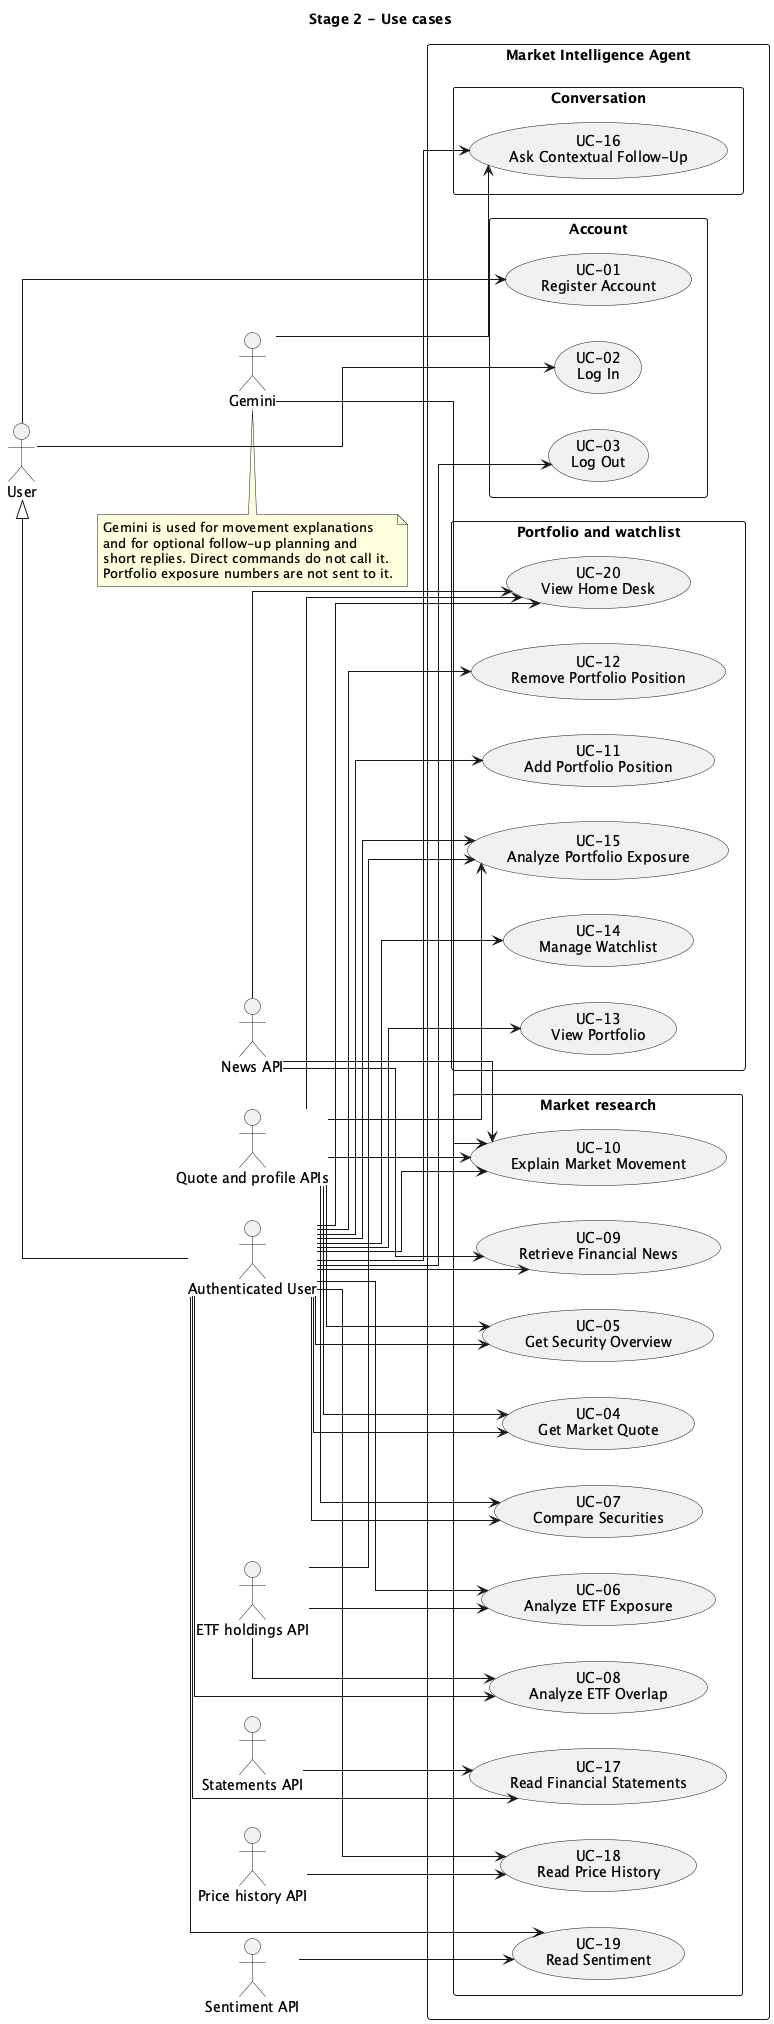
\includegraphics[width=\textwidth,height=0.78\textheight,keepaspectratio]{use-case-diagram.png}
\caption{Use cases. Gemini is associated only with movement explanation and follow-up.}
\end{figure}

\begin{figure}[ht]
\centering
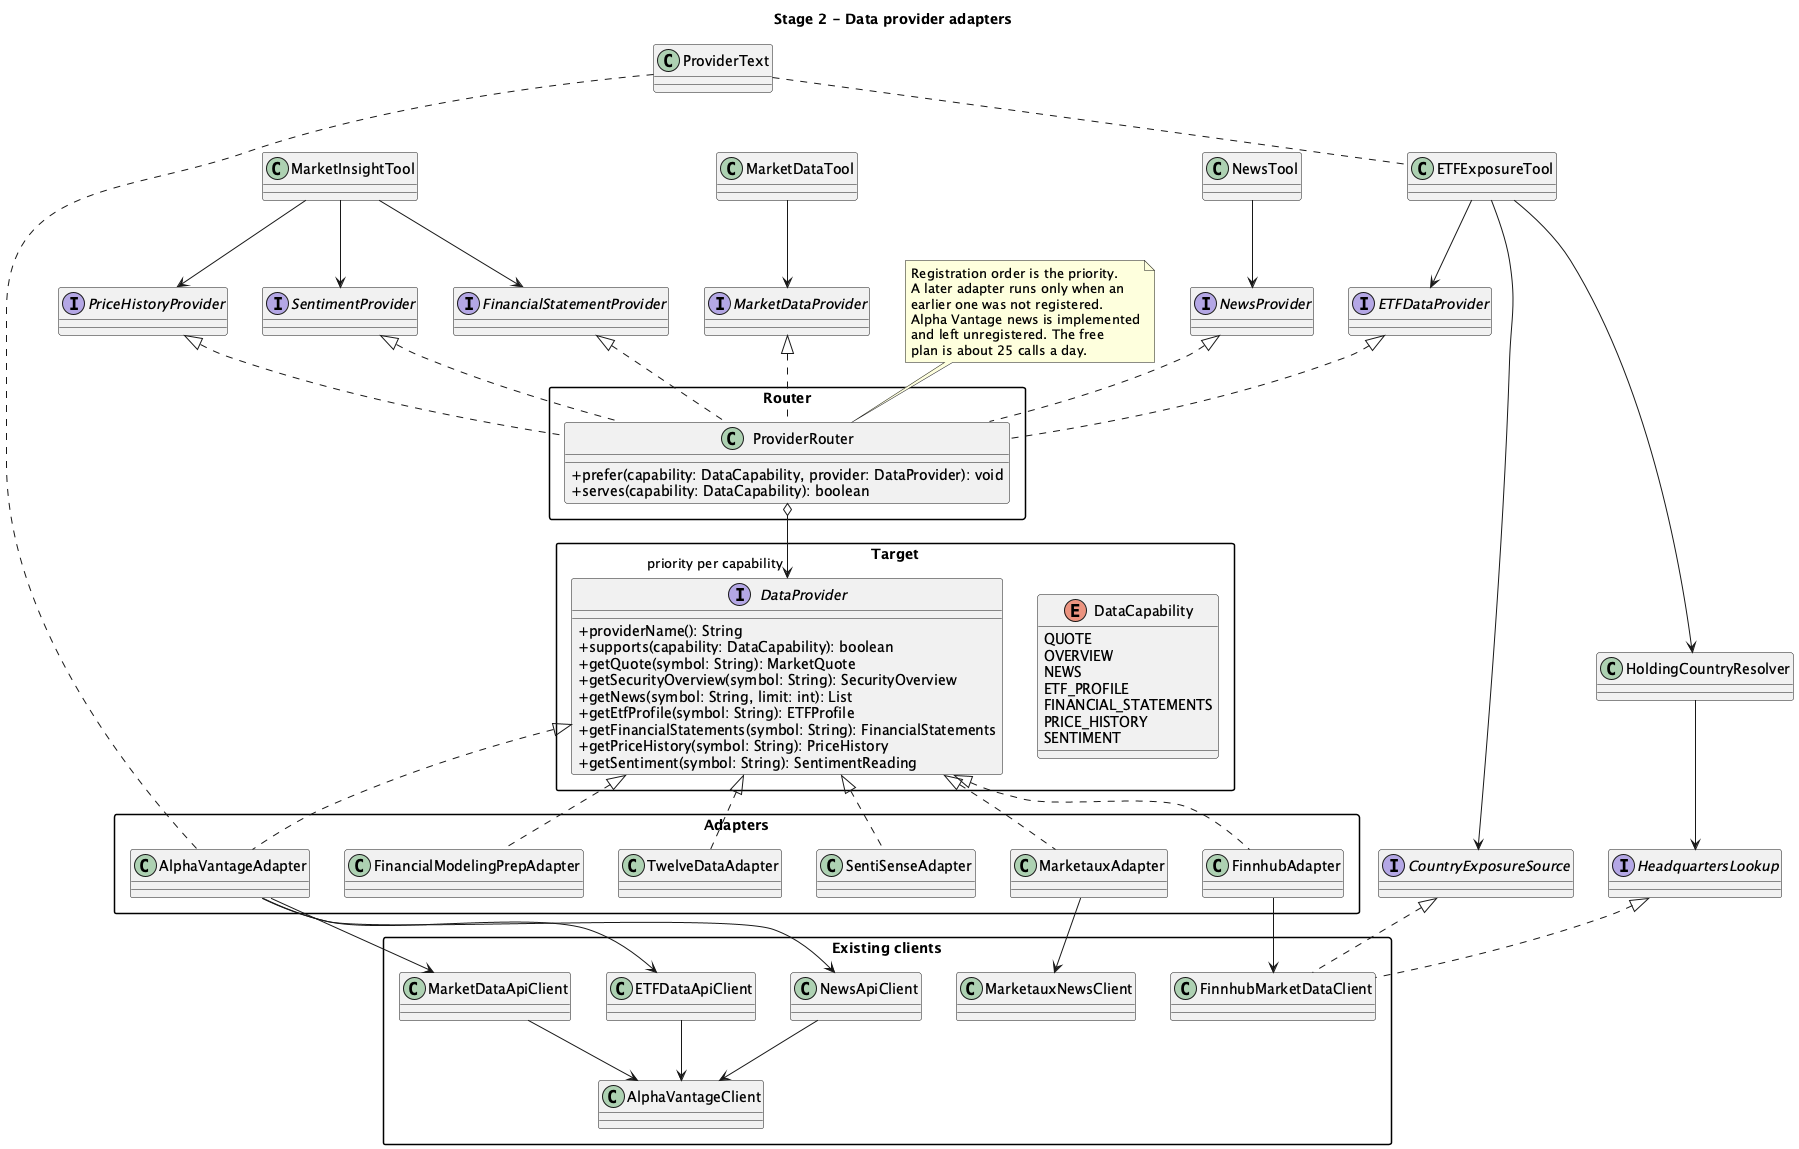
\includegraphics[width=\textwidth,height=0.72\textheight,keepaspectratio]{class-diagram-providers.png}
\caption{Provider adapters and \texttt{ProviderRouter}.}
\end{figure}

\begin{figure}[ht]
\centering
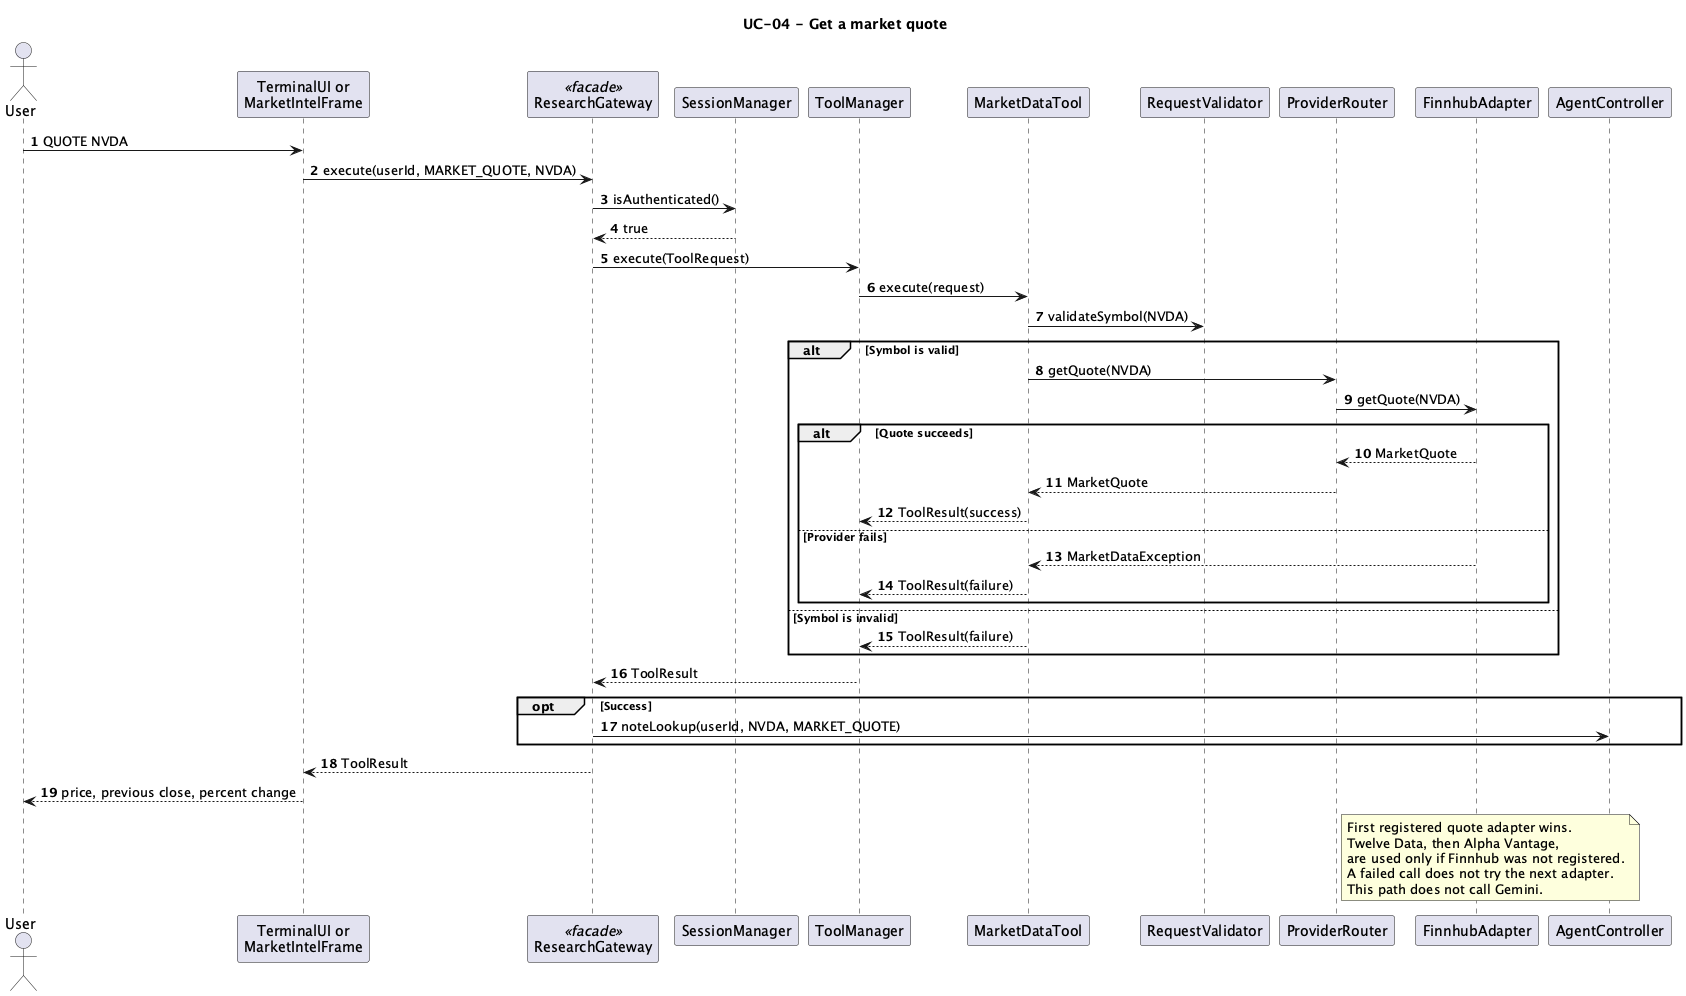
\includegraphics[width=\textwidth,height=0.42\textheight,keepaspectratio]{sequence-market-quote.png}
\caption{UC-04. A quote is a tool call. The model is not on this path.}
\end{figure}

\begin{figure}[ht]
\centering
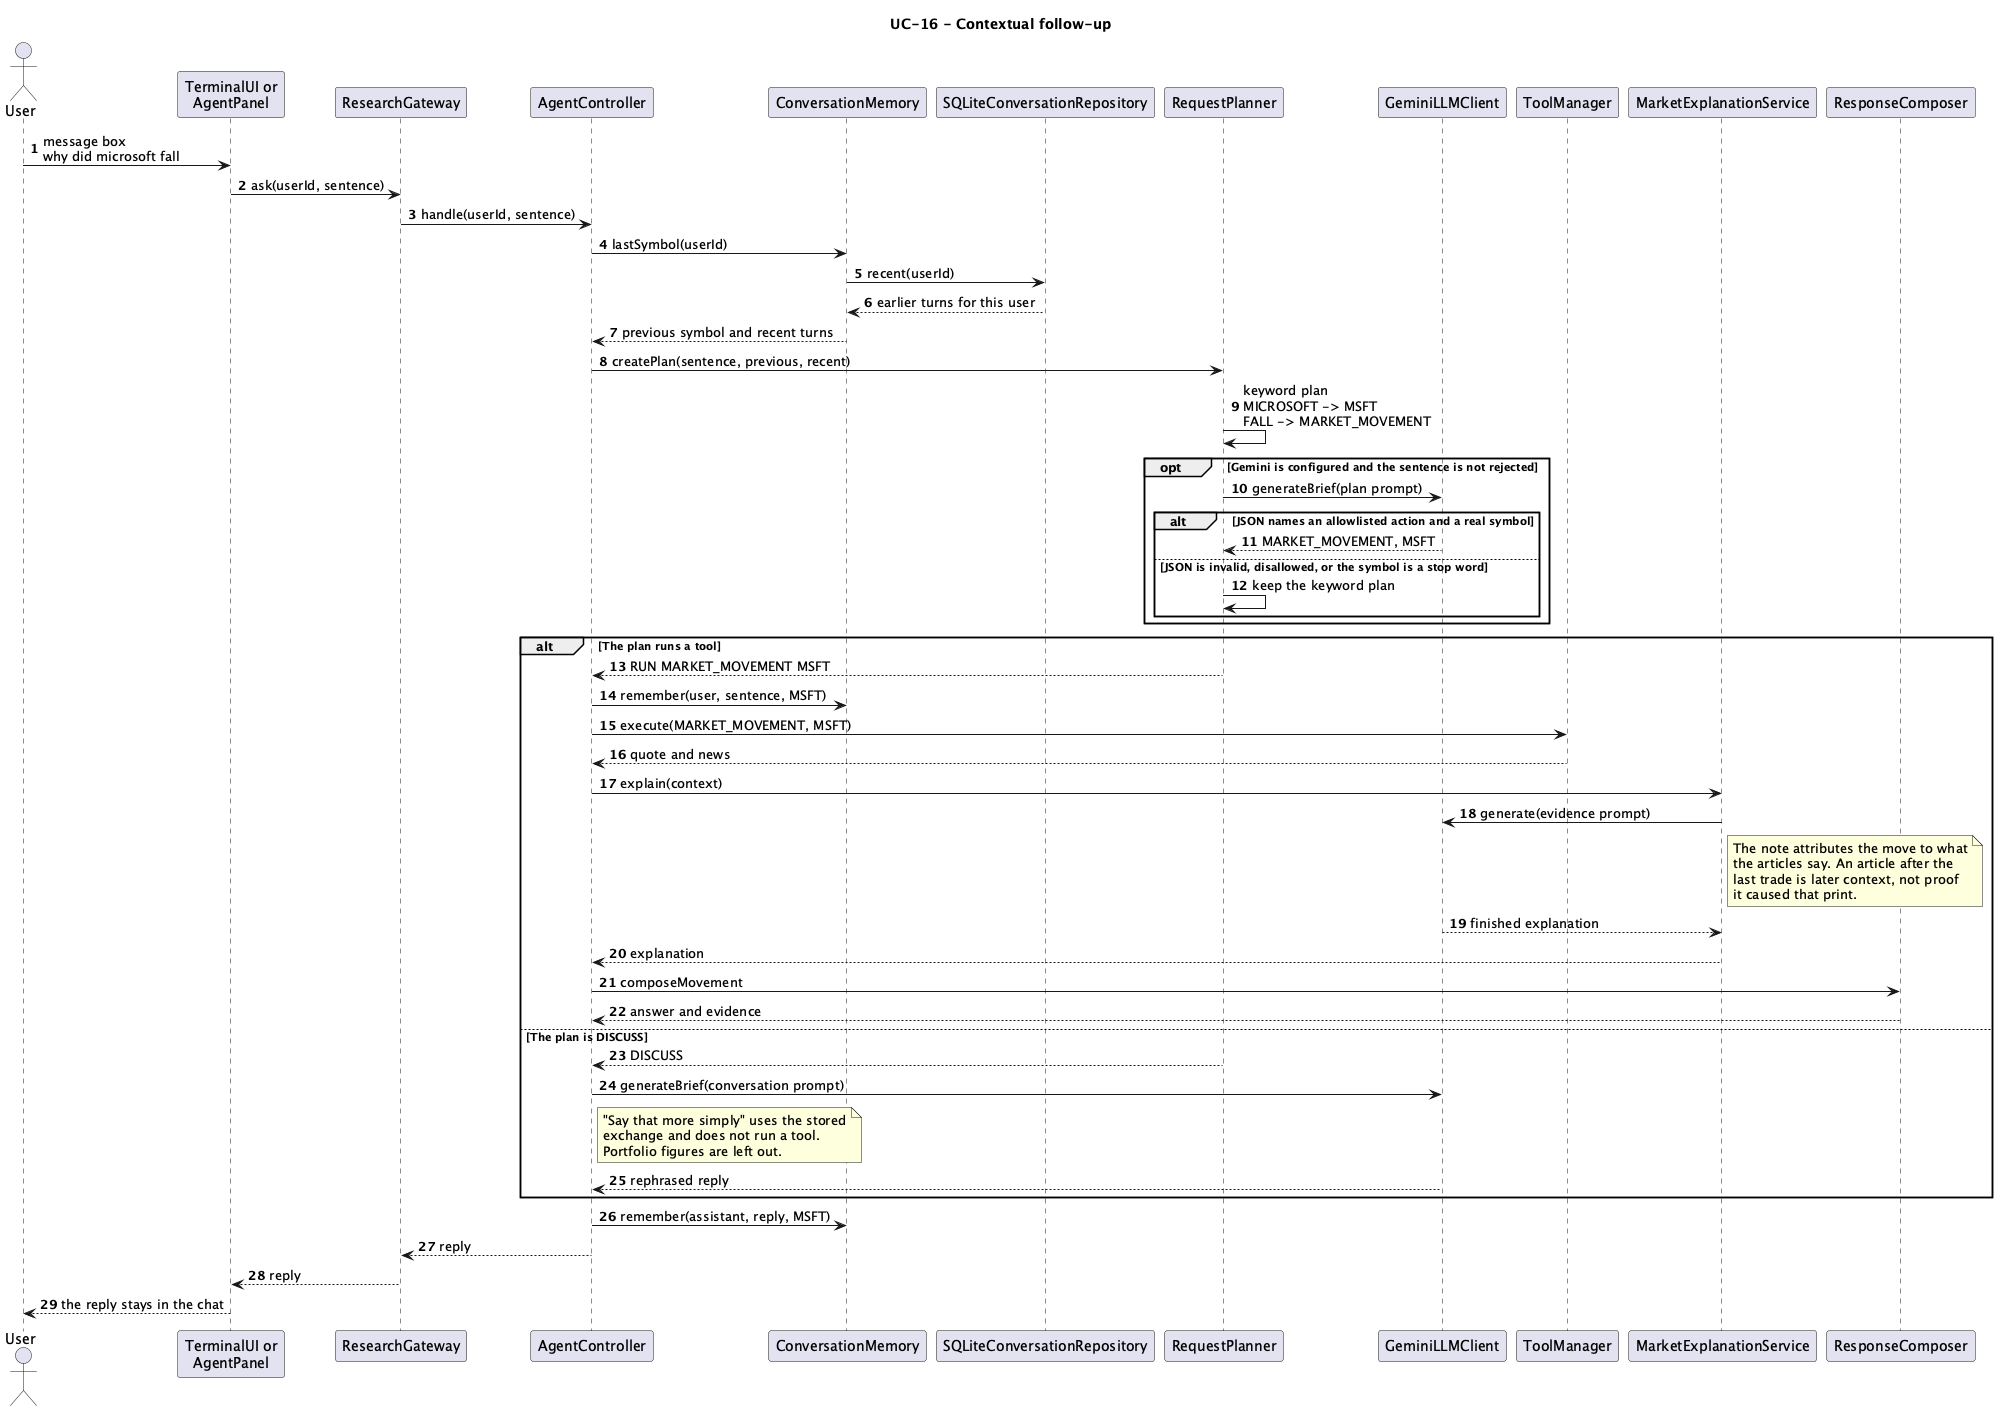
\includegraphics[width=\textwidth,height=0.62\textheight,keepaspectratio]{sequence-context-followup.png}
\caption{UC-16. A sentence is planned against the allowlist, then one tool runs.}
\end{figure}

\begin{figure}[ht]
\centering
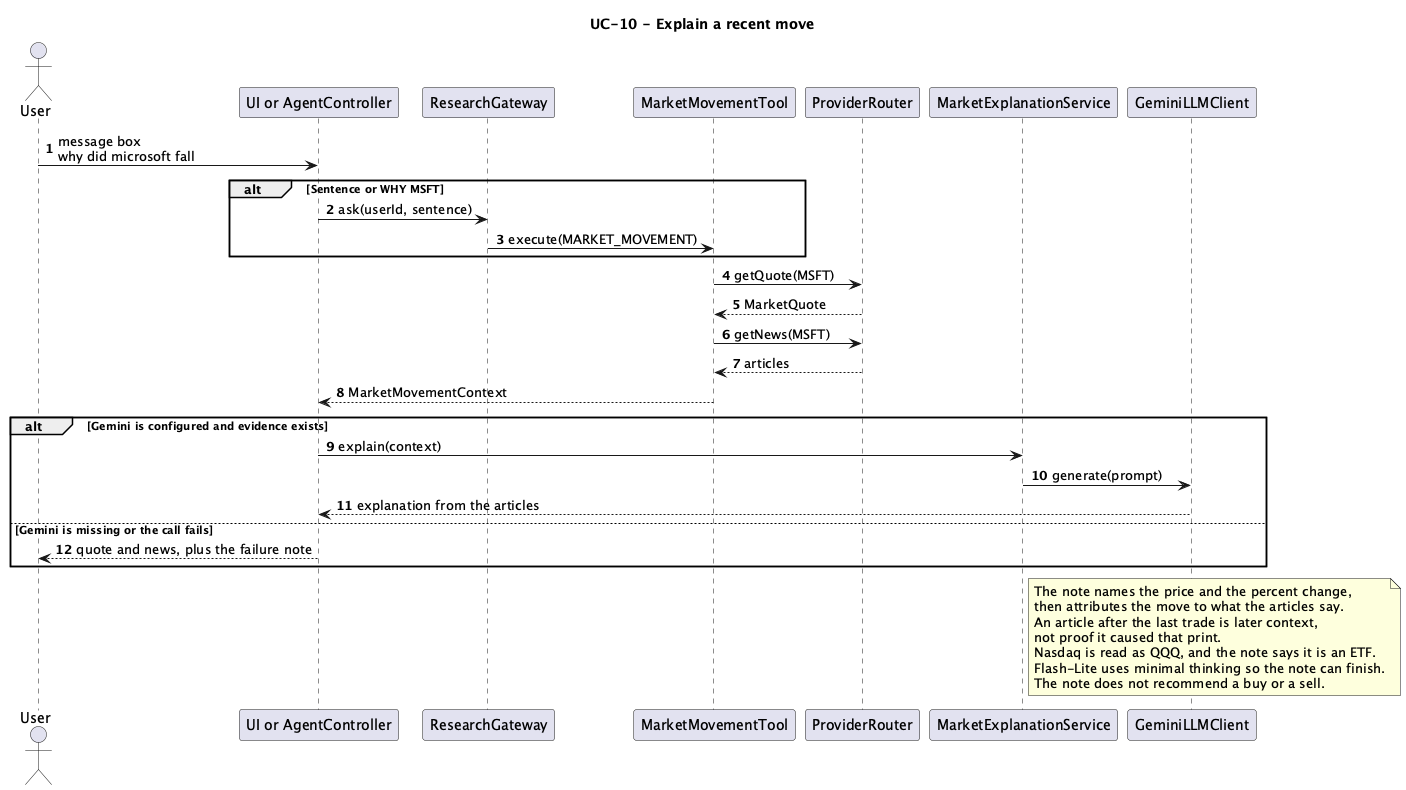
\includegraphics[width=\textwidth,height=0.48\textheight,keepaspectratio]{sequence-market-movement.png}
\caption{UC-10. The quote and the news are gathered first. Gemini writes from that evidence.}
\end{figure}

The remaining PlantUML sources are the class diagrams for the agent, the domain, and persistence, and the sequence diagrams for ETF analysis, country exposure, portfolio analysis, and market insight. Rendered copies are in \texttt{docs/uml/rendered/}.

\section{Development and Verification}

Dates are Toronto local dates of the commits on the public repository. A merge commit is not counted as the meaningful change. The meaningful change is the commit it merged.

\subsection{Weekly Commits}
Period~1, 20--26 October 2026, has no commits. This period does not meet the minimum of five meaningful code commits. The course applies one 5-point deduction when any period misses the minimum. Extra commits in Period~2 do not repair Period~1.

Period~2, 27 October--2 November 2026, has more than five meaningful code commits. Five of them are enough to meet the minimum.

\begin{itemize}
\item \texttt{3770181} -- 28 October. Share service wiring for the terminal and the window.
\item \texttt{f103405} -- 28 October. Swing window over the existing services.
\item \texttt{fcd3877} -- 29 October. Portfolio exposure from price times quantity.
\item \texttt{4da99b3} -- 29 October. Route free APIs through adapters.
\item \texttt{c75e138} -- 29 October. Follow-up from the last stored symbol.
\end{itemize}

Also in Period~2: \texttt{6843eed} Finnhub quotes, \texttt{9716283} country exposure without echoing keys, \texttt{cc386c7} last-trade time, \texttt{1f4db1c} home summary and tape, \texttt{04de078} Gemini interpretation of questions, \texttt{4f52ca0} Flash-Lite, and \texttt{931ec38} so that ``why did microsoft fall'' stays a question.

Period~3, 3--9 November 2026, has six non-merge commits. Five of them change the desk and meet the minimum of five meaningful code commits. This report does not count Period~2 commits toward that week.

\begin{itemize}
\item \texttt{44080fd} -- 5 November. Stage 2 report set in the Stage 1 layout.
\item \texttt{d5d220c} -- 5 November. Home-desk view of value, weight, and unpriced names.
\item \texttt{cfe059e} -- 5 November. Holdings in the center of the home desk.
\item \texttt{9fff4a7} -- 6 November. Background quote refresh keeps the follow-up symbol.
\item \texttt{1bcaa63} -- 6 November. One in-flight quote shared by the tape and the home book.
\item \texttt{a0838f5} -- 6 November. Provider or database reason for an unpriced or unsaved holding.
\end{itemize}

\subsection{Checks}
On 29~October 2026, \texttt{./mvnw test} completed with 207 tests, 0 failures, 0 errors, and 1 skipped. The skipped test is \texttt{GeminiLiveSmokeTest}. It runs only when \texttt{RUN\_GEMINI\_LIVE\_TEST=1} and \texttt{GEMINI\_API\_KEY} are set. The suite uses fake providers and does not call Finnhub, Alpha Vantage, Marketaux, Financial Modeling Prep, Twelve Data, SentiSense, or Gemini.

The owner also ran the Swing desk against live keys. Those sessions found the defects below. They are not a substitute for the automated suite, and the automated suite is not a substitute for a live key.

\subsection{Defects Found and Corrected}
The country request used a URL that returned HTTP 302. It now calls \url{https://api.finnhub.io/api/v1/etf/country}. HTTP 403 on that report was described as a rejected key. The free plan does not include the report. Quotes still work, and the message says so.

An Alpha Vantage notice included the live key. \texttt{ProviderText.redact} replaces that notice. The key was rotated and is not in this report.

\texttt{gemini-3.8-flash} exceeded the explanation timeout. \texttt{gemini-2.5-flash} returned HTTP 404 for a new key. The default is \texttt{gemini-3.5-flash-lite}, with a short token cap and low thinking.

\texttt{why did microsoft fall} was parsed as \texttt{WHY DID}. A multi-word why sentence is now a follow-up. \texttt{WHY MSFT} is still the symbol command.

A movement failure was labeled as an action with no follow-up view. The failure text from the tool is shown instead. Conversation tests failed a foreign key until they inserted the user first. The home screen packed the tiles under a tall empty pane. The summary and the tape were given the room, and the note area was shortened.

Full deterministic testing and KUMA validation remain Stage~3 work, as the Stage~2 instructions say.

\section{AI Collaboration}

Exact token counts were not exported from Cursor or from the Gemini console into this repository. No paid Gemini invoice was recorded for this project. The figures below are therefore not recorded. They are not a claim that the cost was zero in every billing system the student might have elsewhere. Cursor was used on the student's IDE subscription.

\begin{center}
\small
\begin{tabularx}{\textwidth}{@{}p{2.6cm}Xp{2.8cm}@{}}
\toprule
Tool & What it was used for & Cost \\
\midrule
Cursor IDE agent, Grok 4.7 in the Stage~2 sessions. \\
& Java implementation, tests, UML, the README, and this report. The project owner reviewed the running window and rejected behavior that was wrong. \\
& Not exported. Included in the Cursor subscription. No separate invoice is stored here. \\
\addlinespace
ChatGPT, model not named in the log for Interactions 001 and 003. \\
& Stage~1 architecture and the first market-data tool sketch: \texttt{AgentTool}, provider interfaces, and repositories. \\
& Not recorded. \\
\addlinespace
Gemini API in the running desk. The default model is Flash-Lite. \\
& Movement notes and optional follow-up planning and short replies. Not used for quotes, exposure arithmetic, or portfolio edits. \\
& Not exported. No paid invoice recorded. Development calls used the free tier. \\
\bottomrule
\end{tabularx}
\end{center}

The longer log is \texttt{docs/ai-collaboration-log.md}. The interactions that changed the implementation are these.

Interactions 001 and 003. ChatGPT proposed the tool and provider split. The project owner added accounts, portfolios, SQLite, and \texttt{BigDecimal}. That split is still the package layout.

Interaction 004. After Alpha Vantage declined a free educational plan, the owner required one adapter per vendor. Cursor added \texttt{DataProvider} and \texttt{ProviderRouter}.

Interaction 005. The owner saw HTTP 403 on country exposure and then saw an API key in an Alpha Vantage error. The agent added the headquarters fallback and \texttt{ProviderText.redact}. The owner rotated the key.

Interaction 006. The owner reported that ordinary questions were missed, that Gemini timed out, that a new key received HTTP 404 from \texttt{gemini-2.5-flash}, and that ``why did microsoft fall'' was read as the ticker \texttt{DID}. The agent added memory, the allowlist, \texttt{generateBrief}, Flash-Lite, and the sentence parser. The owner confirmed the Microsoft question in the window.

Interaction 007. This report and the updated diagrams. Videos with public links remain the owner's work.

The owner's instruction was that the model should interpret a question, and the answer should come from the tool result. The implementation does that only for an allowlisted action. A sentence that says to ignore previous instructions does not run a tool. That boundary was a human decision, kept after the model was wired in.

\section{Demonstration Index}
\label{sec:demos}

No public video link is in this version of the report. Slides are not a demonstration. Before the 10~November 2026 submission, each row that the course requires needs a public link and a timestamp. Record the running application. Show the GUI and the terminal across the set. Do not show API keys, a \texttt{.env} file, or a shell line that prints a key. If a provider error appears, confirm the key is not on screen.

On 5~November 2026 two recordings were made on this machine, with no provider keys set. They are not public links, and they do not show live vendor data.

The window recording creates account \texttt{erdem}, returns to sign-on, rejects the password \texttt{wrong-pass} with ``Invalid username or password.'', signs in, opens the home desk, saves \texttt{NVDA} as 10 shares of type \texttt{STOCK}, adds \texttt{MSFT} to the monitor, runs \texttt{QUOTE NVDA}, and logs off. The quote result names \texttt{FINNHUB\_API\_KEY}, \texttt{TWELVE\_DATA\_API\_KEY}, and \texttt{ALPHA\_VANTAGE\_API\_KEY}. No price is shown.

The terminal recording signs in as \texttt{erdem}, runs \texttt{/portfolio} (the \texttt{NVDA} row), \texttt{/watchlist} (\texttt{MSFT}), and \texttt{/quote NVDA}. The quote says no tool is registered for \texttt{MARKET\_QUOTE}. The sentence \texttt{why did microsoft fall} is labeled \texttt{FOLLOW-UP MSFT} and reports that the movement tool is not registered. It does not use \texttt{DID} as a ticker. \texttt{/logout} returns to the authentication menu.

Live quote, news, movement, statement, history, and sentiment clips still need the student's keys and a public link.

\begin{center}
\small
\begin{tabularx}{\textwidth}{@{}p{1.5cm}Xp{3.4cm}@{}}
\toprule
Feature & What to show & Link \\
\midrule
UC-01 & GUI create-account screen, confirmation present, then return to sign-on. & Local window recording. No public link. \\
UC-02 & Sign-on screen with no confirmation field. Wrong password, then a successful sign-on. & Local window recording. No public link. \\
UC-03 & Log out and show that the next command requires sign-on. & Local window and terminal recordings. No public link. \\
UC-04 & \texttt{QUOTE NVDA} in the window and \texttt{/quote NVDA} in the terminal. Both show the missing provider. No price. & Local recordings. No public link. \\
UC-05 & \texttt{OVERVIEW NVDA}. Name, exchange, currency, industry. Say that a description is not on the free profile. & Not recorded \\
UC-06 & \texttt{SECTOR QQQ}, then \texttt{GEO QQQ}. Headquarters note, and a stock such as \texttt{NVDA} producing no country list. & Not recorded \\
UC-07 & \texttt{COMPARE NVDA MSFT}. Difference of percent changes. & Not recorded \\
UC-08 & \texttt{OVERLAP QQQ SPY}. Shared holdings. & Not recorded \\
UC-09 & \texttt{NEWS NVDA}. Say that a match is not a cause. & Not recorded \\
UC-10 & \texttt{WHY MSFT}. Quote, news, Gemini note, and the not-advice line. & Not recorded \\
UC-11 & \texttt{PORT ADD NVDA 10 STOCK} or the Portfolio screen. & Local window recording. No public link. \\
UC-12 & Remove a symbol that exists, then one that does not. & Not recorded \\
UC-13 & \texttt{/portfolio} and the Portfolio screen for the same user. & Local terminal recording. No public link. \\
UC-14 & \texttt{WATCH ADD} and \texttt{WATCH REMOVE}. & Add recorded. Remove not recorded. \\
UC-15 & \texttt{EXPOSURE}. Value as price times quantity. Name an unpriced position if one exists. & Not recorded \\
UC-16 & After a lookup, ask ``what about its sector exposure.'' Then ``why did microsoft fall,'' and show \texttt{MSFT}, not \texttt{DID}. Then a sentence that says to ignore previous instructions. & The Microsoft sentence is in the local terminal recording. The other two sentences are not recorded. \\
UC-17 & \texttt{STATEMENTS NVDA}, or the unavailable message when the key is unset. & Not recorded \\
UC-18 & \texttt{HISTORY NVDA}. Bars and RSI. & Not recorded \\
UC-19 & \texttt{SENTIMENT NVDA}. Score and band. Say the band is not advice. & Not recorded \\
UC-20 & F1 after sign-on. Portfolio value, day move, chips, and the tape. GUI only. & Home appears after sign-on in the local window recording. The tape has no quotes. \\
\bottomrule
\end{tabularx}
\end{center}

The terminal segment should include \texttt{/quote}, \texttt{/why} or a follow-up sentence, and \texttt{/portfolio exposure}. The window segment should include sign-on, home, and at least one research command. Together they show both interfaces.

\section{Stage 2 Summary}
The Stage~1 design is now a running desk. Both interfaces call one gateway. Research actions are commands. Vendor payloads sit behind adapters, and \texttt{ProviderRouter} chooses one adapter per capability by registration order. Deterministic Java code performs authentication, persistence, validation, and exposure arithmetic. Gemini writes a movement note from retrieved evidence and may name one allowlisted follow-up action. It does not edit the portfolio, and a quote does not call it.

What remains before the 10~November 2026 submission is public demonstration links for the rows in Section~\ref{sec:demos}. Period~3 has the six non-merge commits listed under Weekly Commits. Period~1 remains a missed week.

\end{document}
